\cleardoublepage
\chapter{Application game screens}
\label{apdx:gamescreens}

This appendix shows all the screens which conform the application. It goes through the three different game modes and shows all the screens contained within them.

\cleardoublepage

\section{Home}

\begin{figure}[ht!]
  \centering
  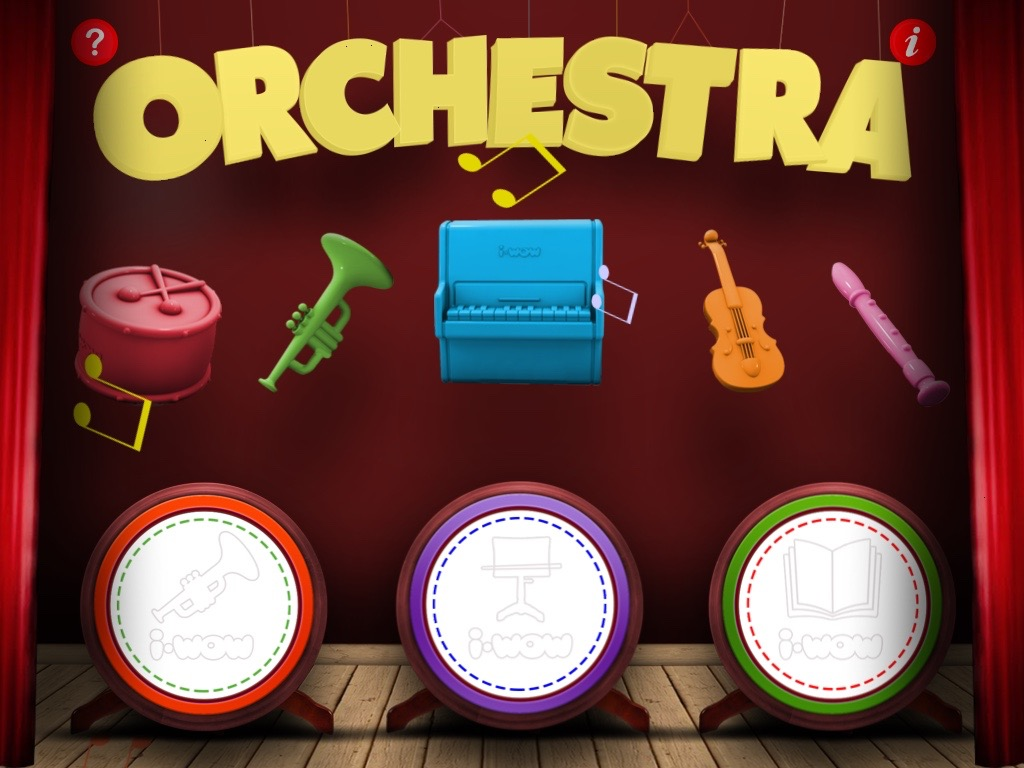
\includegraphics[width=350pt]{graphics/use-case/home_screen.jpg}
  \vspace{0.05cm}
  \caption{Application Home Screen}
  \label{fig:home_screen}
  \vspace{0.6cm}

  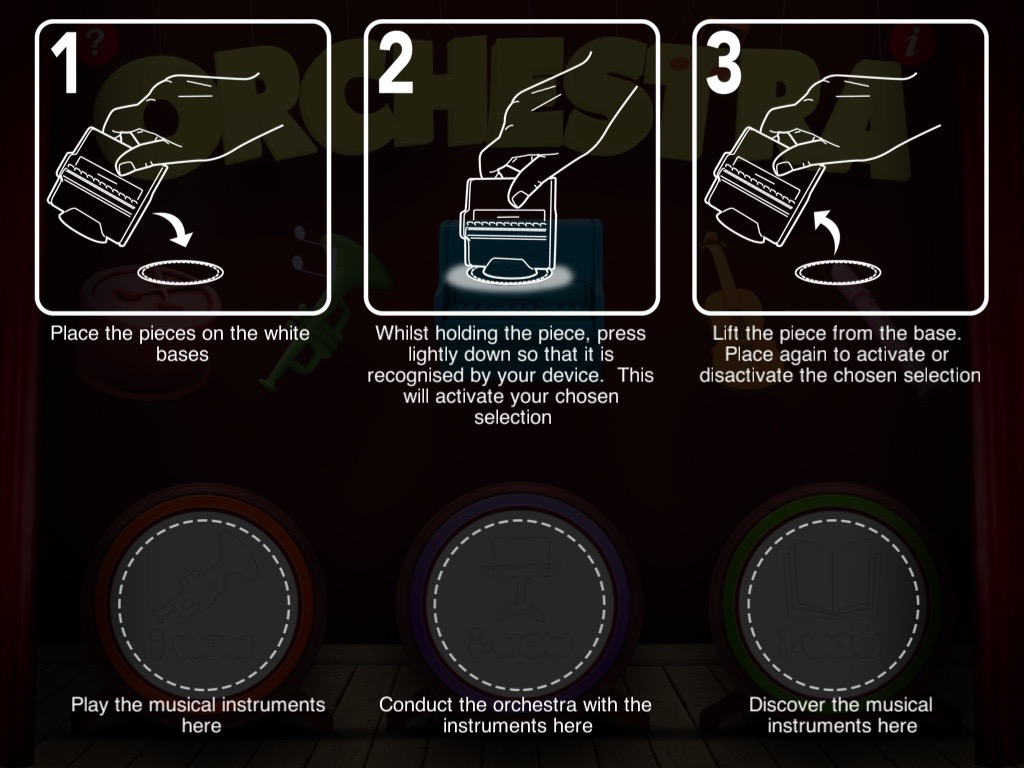
\includegraphics[width=350pt]{graphics/use-case/help_home_screen.jpg}
  \vspace{0.05cm}
  \caption{Help Home Screen}
  \label{fig:help_home_screen}
\end{figure}

\section{Playing game mode}

\begin{figure}[ht!]
  \centering
  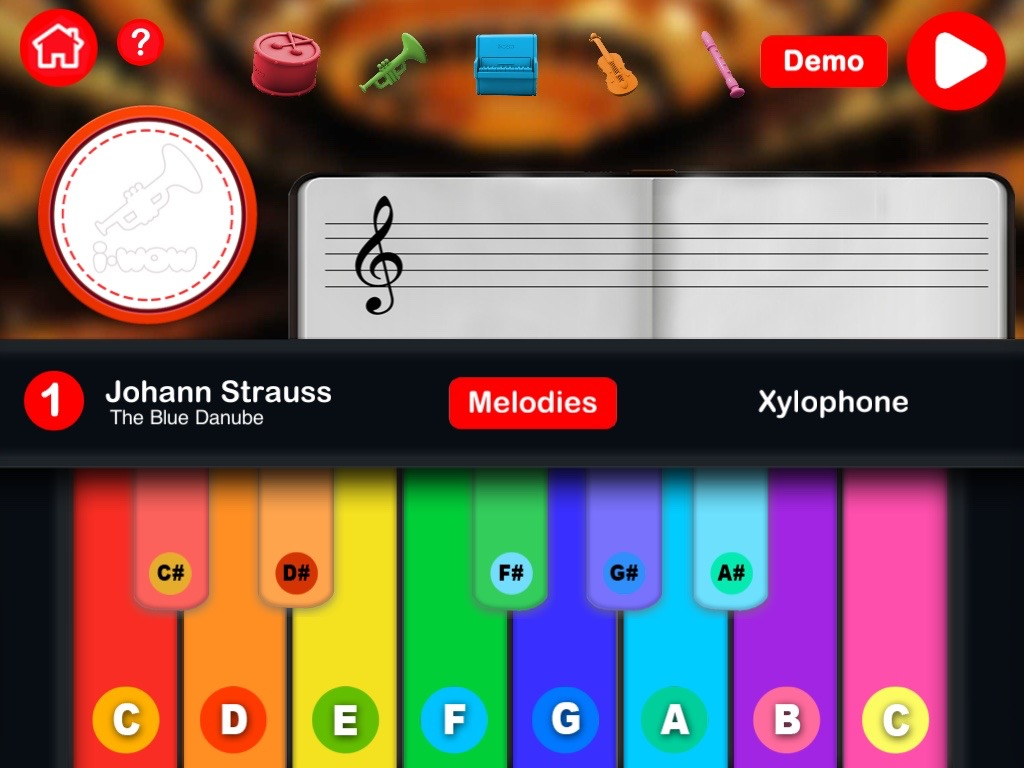
\includegraphics[width=350pt]{graphics/use-case/playing_xylo_start_screen.jpg}
  \vspace{0.05cm}
  \caption{Xylophone playing instrument game mode}
  \label{fig:playing_xylo_start_screen}
  \vspace{0.6cm}

  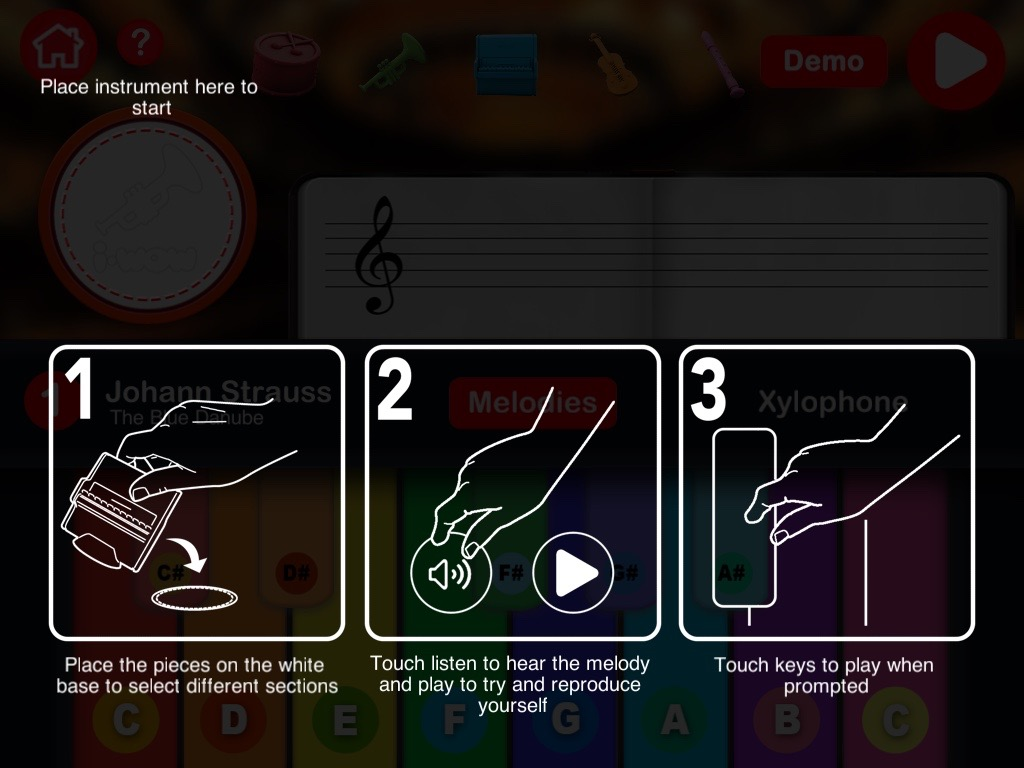
\includegraphics[width=350pt]{graphics/use-case/help_playing_screen.jpg}
  \vspace{0.05cm}
  \caption{Help information playing instrument game mode}
  \label{fig:help_playing_screen}
\end{figure}

\begin{figure}[ht!]
  \centering
  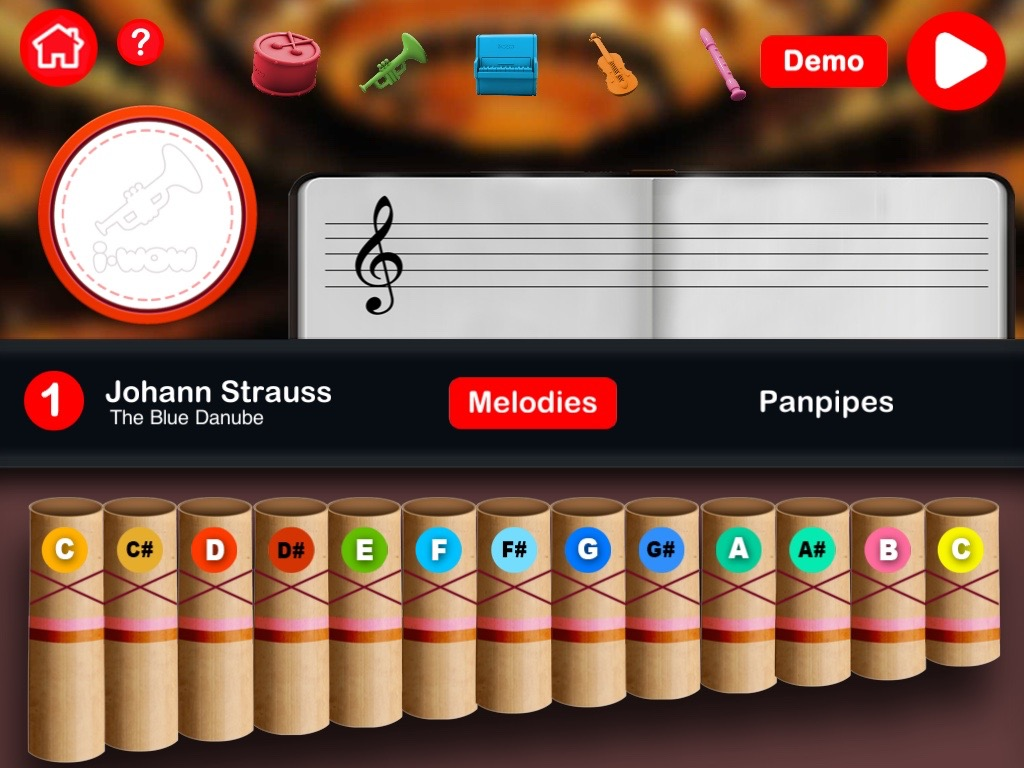
\includegraphics[width=350pt]{graphics/use-case/playing_panpipes_screen.jpg}
  \vspace{0.05cm}
  \caption{Playing panpipes screen}
  \label{fig:playing_panpipes_screen}
  \vspace{0.6cm}

  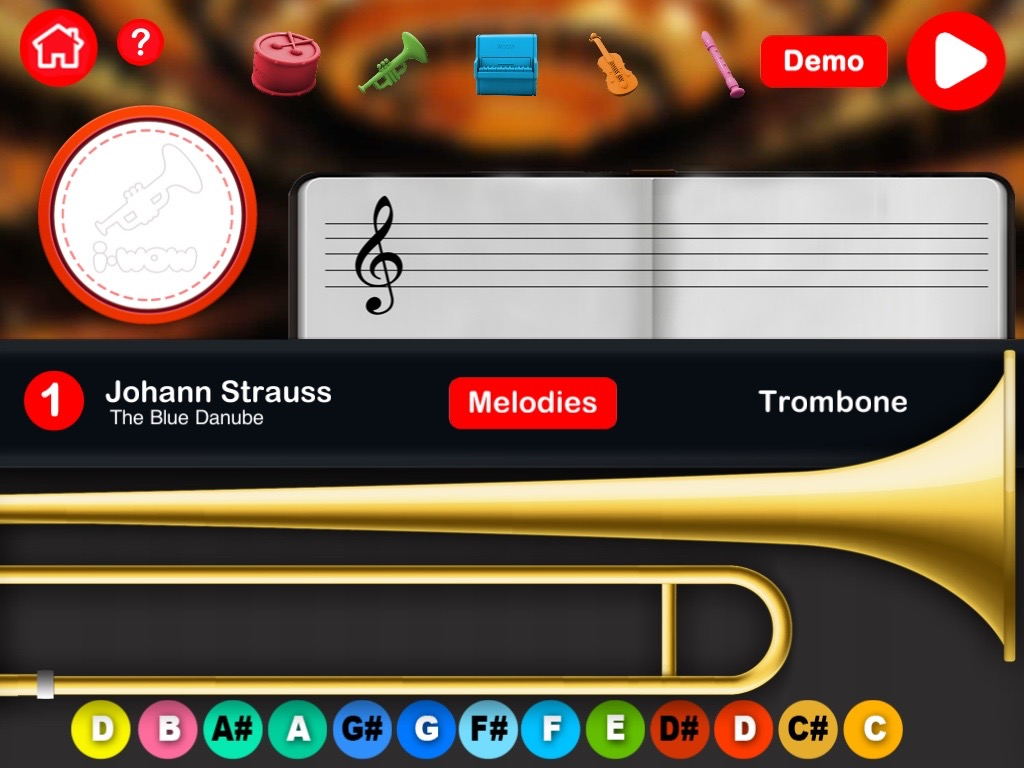
\includegraphics[width=350pt]{graphics/use-case/playing_trombone_screen.jpg}
  \vspace{0.05cm}
  \caption{Playing trombone screen}
  \label{fig:playing_trombone_screen}
\end{figure}

\begin{figure}[ht!]
  \centering
  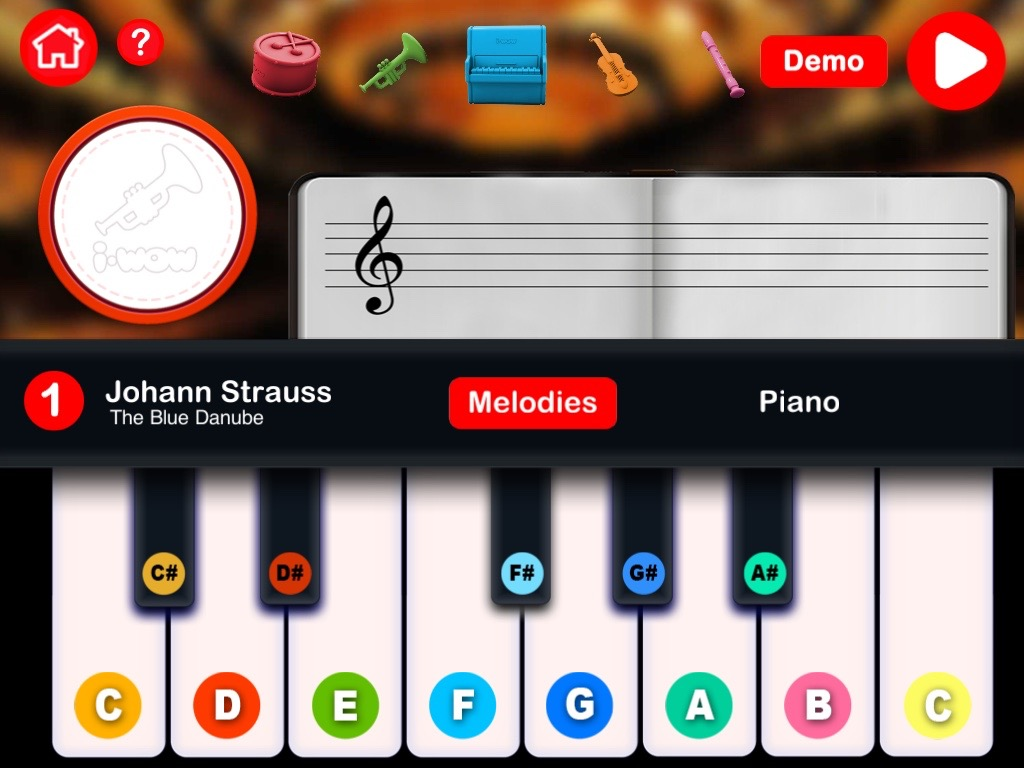
\includegraphics[width=350pt]{graphics/use-case/playing_piano_screen.jpg}
  \vspace{0.05cm}
  \caption{Playing piano screen}
  \label{fig:playing_piano_screen}
  \vspace{0.6cm}

  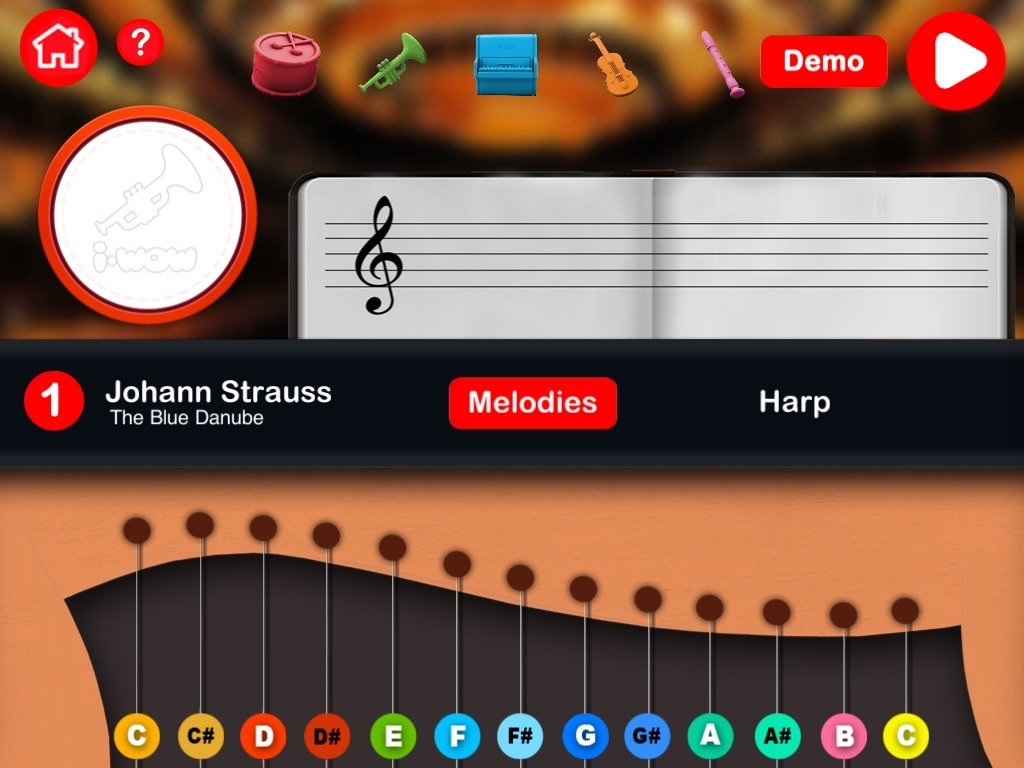
\includegraphics[width=350pt]{graphics/use-case/playing_harp_screen.jpg}
  \vspace{0.05cm}
  \caption{Playing harp screen}
  \label{fig:playing_harp_screen}
\end{figure}

\section{Conducting game mode}

\begin{figure}[ht!]
  \centering
  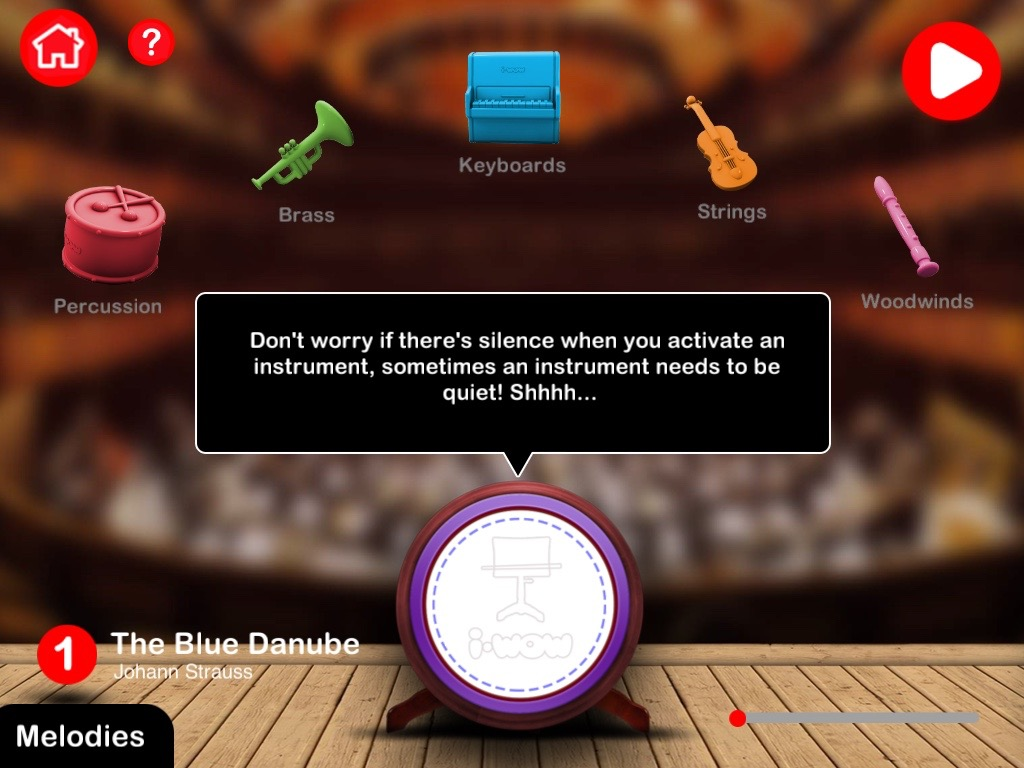
\includegraphics[width=350pt]{graphics/use-case/conducting_home_screen.jpg}
  \vspace{0.05cm}
  \caption{Conducting game mode access screen}
  \label{fig:conducting_home_screen}
  \vspace{0.6cm}

  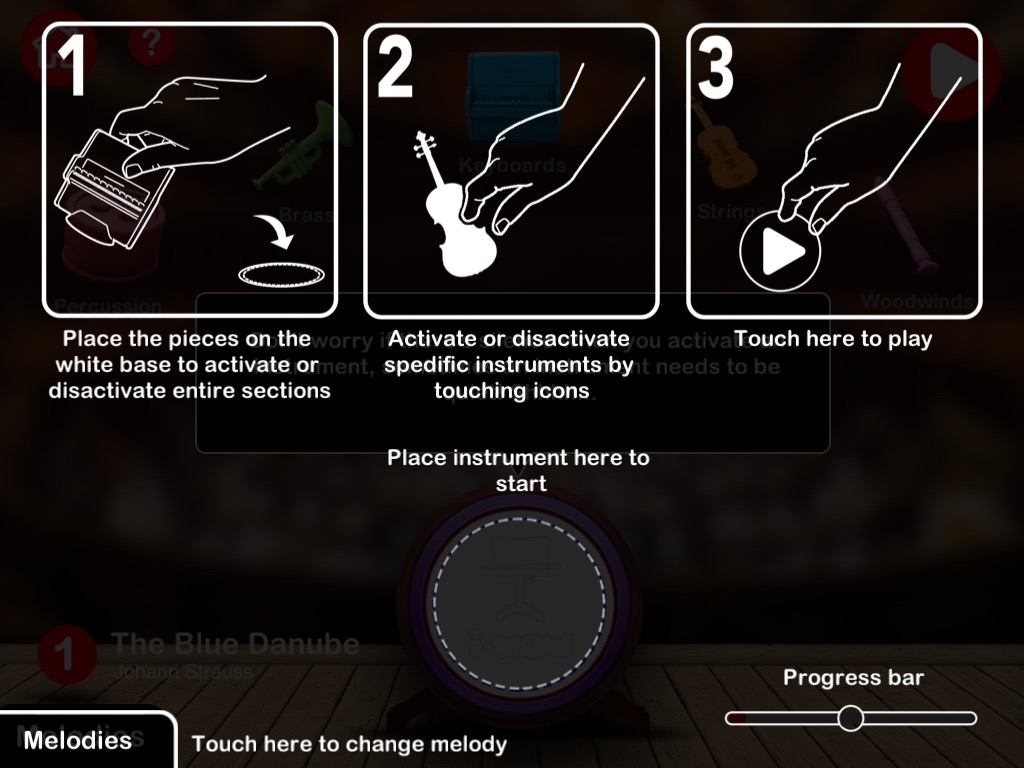
\includegraphics[width=350pt]{graphics/use-case/help_conducting_screen.jpg}
  \vspace{0.05cm}
  \caption{Help information conducting orchestra game mode}
  \label{fig:help_conducting_screen}
\end{figure}

\begin{figure}[ht!]
  \centering
  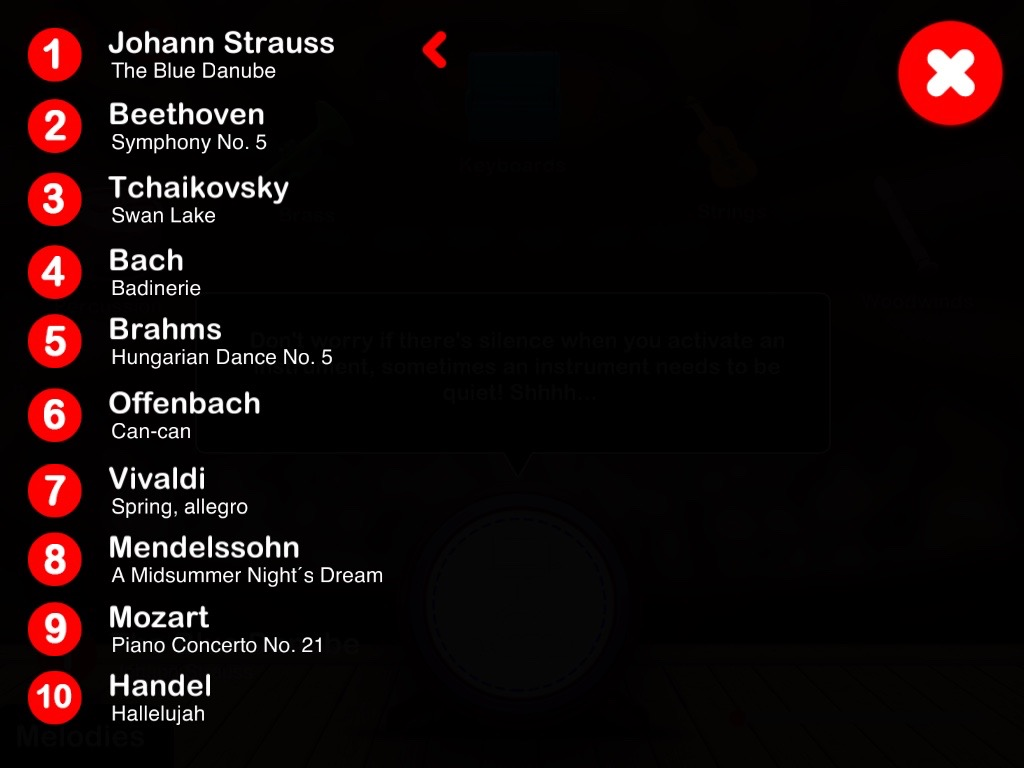
\includegraphics[width=350pt]{graphics/use-case/conducting_melodies_screen.jpg}
  \vspace{0.05cm}
  \caption{Melodies selection in the conducting orchestra game mode}
  \label{fig:conducting_melodies_screen}
  \vspace{0.6cm}

  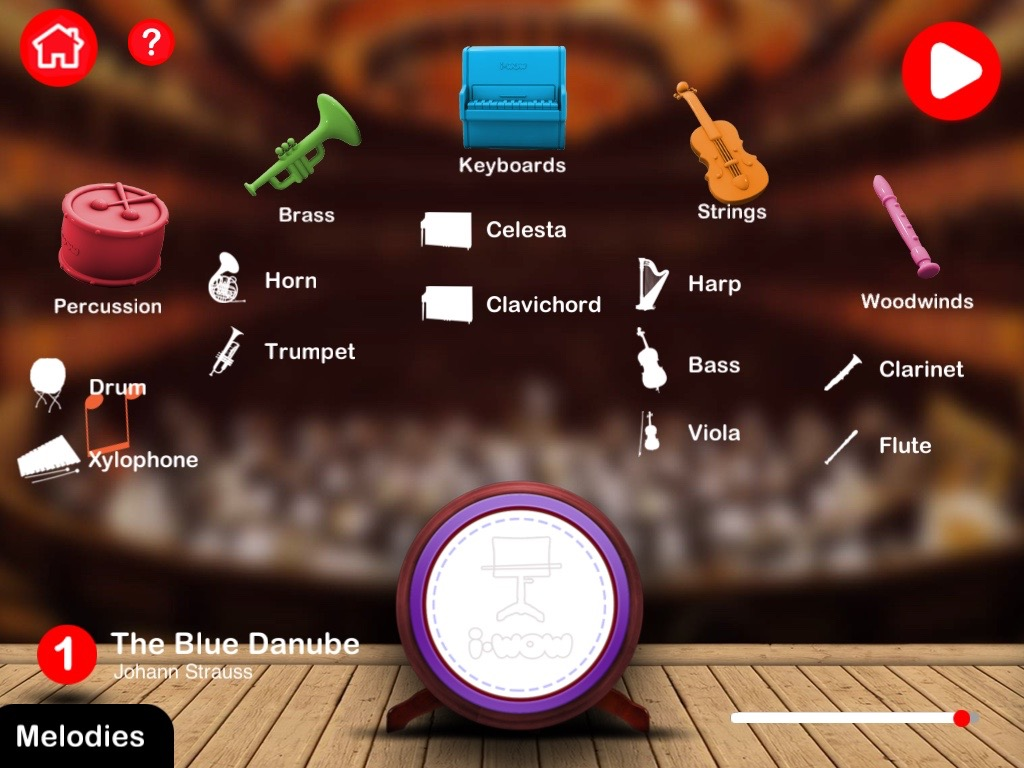
\includegraphics[width=350pt]{graphics/use-case/conducting_all_stop_screen.jpg}
  \vspace{0.05cm}
 \caption{Conducting orchestra screen with all instruments activated}
  \label{fig:conducting_all_stop_screen}
\end{figure}

\section{Discovering game mode}
